\begin{frame}{\citetitle{MarcoNuno_CongArbEsp_2013_11_01} \footnotemark (1)}
%\begin{block}{Prototipo de un entorno virtual para un robot de servicio\footnotemark } 
\begin{columns}
\begin{column}{0.52\textwidth}
    \begin{center}

\begin{itemize}
\item Prototipo SerBot I
\item Modelo 3D del Robot
\item Modelo 3D del entorno
\item Plataforma: PC de escritorio
\end{itemize}
     \end{center}

\end{column}
\begin{column}{0.48\textwidth}  
    \begin{center}
\begin{itemize}
\end{itemize}
     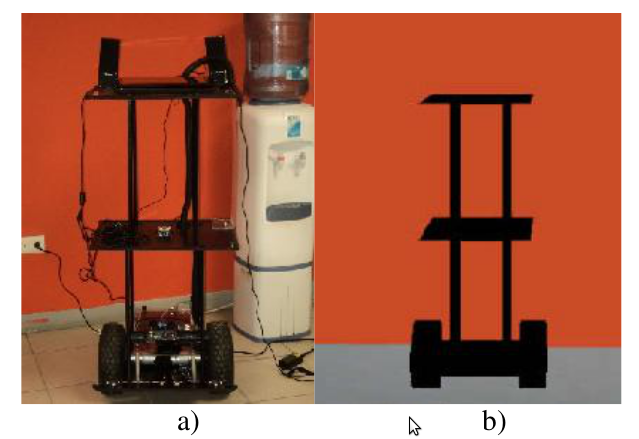
\includegraphics[width=0.9\textwidth]{Figs/SerbotI_A}\\
     \end{center}
\end{column}
\end{columns}


%\end{block} 
\footnotetext{\fullcite{MarcoNuno_CongArbEsp_2013_11_01}}
%\\setcounter{footnote}{0}
\end{frame}



\begin{frame}{\citetitle{MarcoNuno_CongArbEsp_2013_11_01} (2)}
%\begin{block}{Prototipo de un entorno virtual para un robot de servicio (2)} 
\begin{columns}
\begin{column}{0.60\textwidth}
    \begin{center}

\begin{itemize}
\item A partir de los planos de los edificios y de las fotografías, se construyó un prototipo del entorno
\item El plano permitía determinar en donde esta ubicadas paredes y puertas
\end{itemize}
     \end{center}

\end{column}
\begin{column}{0.38\textwidth}  
    \begin{center}
\begin{itemize}
\end{itemize}
     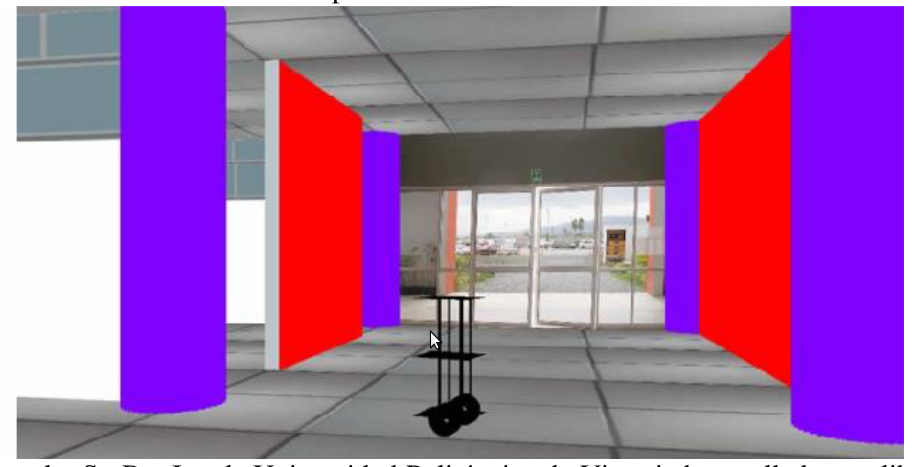
\includegraphics[width=0.9\textwidth]{Figs/SerbotI_B}\\
     \end{center}
\end{column}
\end{columns}
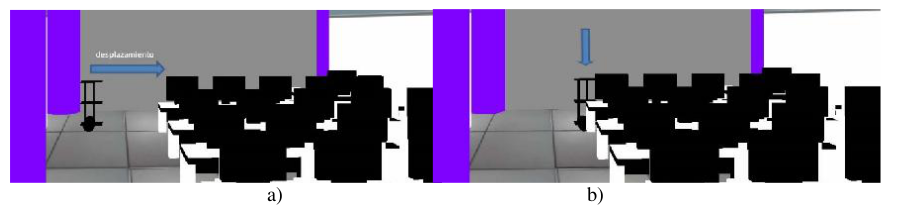
\includegraphics[width=0.8\textwidth]{Figs/SerbotI_C}\\


%\end{block} 
\end{frame}


\begin{frame}{\citetitle{MarcoNuno_CongArbEsp_2013_11_01} (3)}
%\begin{block}{Prototipo de un entorno virtual para un robot de servicio (2)} 
\begin{columns}
\begin{column}{0.48\textwidth}
    \begin{center}

\begin{itemize}
\item Se implementarion controles para movimiento del Robot y del cambio de Vista
\item En robot podía avanzar hacia adelante (moviendo las ruedas en la misma dirección) pero girar moviendo una rueda y dejando la otra quieta
\end{itemize}
     \end{center}

\end{column}
\begin{column}{0.52\textwidth}  
    \begin{center}
\begin{itemize}
\end{itemize}
     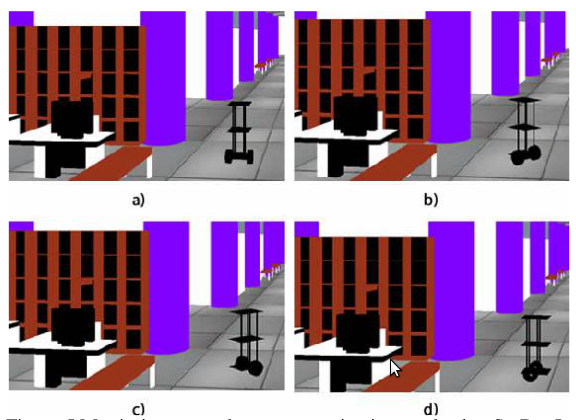
\includegraphics[width=0.9\textwidth]{Figs/SerbotI_D}\\
     \end{center}
\end{column}
\end{columns}
%\end{block} 
\end{frame}
